\documentclass[10pt,letterpaper]{article}
\usepackage{style/tmlr}
\usepackage{amsmath,amssymb,booktabs,graphicx,hyperref}
\hypersetup{hidelinks,pdftitle={Supplement: Evaluating the Deployment Utility of a Frozen Policy-Update Procedure: Scale, Completion Preference, and Joint Evidence},pdfauthor={}}
\graphicspath{{figures/}}
\title{Supplementary Material for\\Evaluating the Deployment Utility of a Frozen Policy-Update Procedure: Scale, Completion Preference, and Joint Evidence}
\author{Anonymous authors}
\date{}
\begin{document}
\maketitle
\section{Evidence and independent units}
The principal cohort contains 50 independent roots, each shared across two synthetic liquidity regimes. The 100 selection decisions and 2,400 paired deployment repetitions are repeated observations within those roots. The original family contains 24 estimates under a 100 bps incomplete-fill penalty. Root resampling carries both regimes and every cell together. All results remain conditional on the frozen policy generator, selection rule, exogenous population, and matching-world implementation.

The utility diagnostic retains the original policies and outcomes and varies only their valuation at 25, 50, 100, and 200 bps. Its 64-estimate family was defined after the primary outcomes were inspected. Root deletion and alternative-band constructions also reuse the original data after inspection. None of these checks supplies another independent cohort or changes the original 24-estimate family.

The proxy-to-deployment comparison is a separate post-outcome diagnostic at the $s=0.05$ selection scale. It contrasts the selected candidate's saved proxy gain, with no-update decisions set to zero, against the mean of four paired interactive deployment gains under the recorded $U_{100}$ convention. Its four root-level differences use a separate whole-root simultaneous band. This comparison does not identify causal proxy bias and is not part of the original 24-estimate family.

The additional November 4 break-even diagnostic uses the two saved utility components at the largest scale. Its separate specification acknowledges inspection of the earlier results. The eight-component whole-root bootstrap rectangle and its projected nonnegative zero sets retain every root, including no-update zeros. The analysis fixes all original choices; it does not assess re-selection at other completion penalties. Its uncertainty family is separate from the 24- and 64-estimate families.

The planner study contains three generation roots with 32 ordered attempts each and a fixed 20-task deployment panel. Invalid/duplicate attempts retain their positions. Its positive observed means are an auxiliary case with exploratory pointwise uncertainty; they are not evidence for unrestricted agents or an independent model backbone. The full case is reported here rather than in the main evidence section, and its outcomes are not pooled with market roots.

\section{What is inherited and what is separately evidenced}
Improvement Fidelity, reversal summaries, no-update decisions, paired comparisons, and root-bootstrap tools are attributed to related work \citep{pivot} or used as standard statistical operations. PIVOT-KG, its validation-allocation comparisons, the prior response experiments, and its virtual finance fixtures are not contributions of this submission. The primary new evidence is the separately frozen matching-engine cohort; the planner-code study is retained as a bounded supplementary case, with explicitly post-outcome diagnostics.

The matching engine has a different source lineage from the earlier development exchange. Policies, candidate equations, and the completion utility were nevertheless carried forward for compatibility. Implementation lineage does not imply independence from all development choices. The engine's accounting and independent replay checks validate saved synthetic events rather than real-market realism.

An anonymous comparison copy of the actual concurrently reviewed conference manuscript is supplied as \texttt{related\_work/pivot-anonymous.pdf}. It is solely related-work material, not part of the new result set. The originality review also used that submission's separate supplementary archive, which includes older source and virtual execution examples. Its older source version was not silently substituted for the actual conference PDF. The full public reference is retained outside the anonymous review package for restoration after review.

\section{Portable reanalysis and build}
The ZIP contains manuscript sources, normalized outcome data, expected summaries, a data dictionary, dependencies, and a hash inventory. Install \texttt{reproduction/requirements.txt} into an isolated Python environment and run, from the package root:
\begin{verbatim}
bash reproduce_all.sh /path/to/output
\end{verbatim}
The system additionally needs a working TeX installation with \texttt{latexmk}, \texttt{pdflatex}, and \texttt{bibtex}. The Python dependencies are pinned in the package; no model credentials, simulator, original dataset download, or task-fitting runtime is needed for this saved-outcome check.

The wrapper verifies the outcome hashes; reconstructs the original 24 estimates, the 64 diagnostic estimates, the four proxy-to-deployment gaps, and the five planner-prefix summaries; recomputes all 50 root deletions, four alternative bands, and the break-even diagnostic; then generates the tables and vector plots consumed by the manuscript builds. All numeric results are checked against the bound references within $10^{-9}$ in their native units. The build uses the recomputed outputs, not a precompiled PDF. PDF text and numerical agreement are checked separately from rendering bytes.

The break-even output includes the 50-root component data, the eight simultaneous component intervals, the nonnegative zero sets, and denominator-instability counts. No ratio draws are silently dropped. In the two liquid cells, denominator sign changes suppress the simple percentile-ratio summary; the projected component sets remain available. The diagnostic script handles bounded, unbounded, and empty sets and rejects constant empirical components for this standardized construction. Its methods and limitations are detailed in the main-paper appendix.

The original market CSV includes the independent root, regime, adopted candidate, incumbent, proxy gain, paired deployment gain, scale, response, replication index, no-update flag, configuration hash, and the two saved utility components. A complete record key is the tuple of root, regime, response, scale, and repetition. Missing/duplicate keys, nonfinite values, inconsistent selections, nonzero no-update gains, and failed statuses are rejected. A failed attempt is never repaired by replacing the root.

Portable reanalysis does not regenerate model responses, original task fits, or exchange event streams. The raw-event replay and original grade audits are distinct retained evidence. The package establishes that its saved-outcome claims can be reconstructed; it is not a new independent scientific replication. Uncompleted wider-project studies remain excluded from the paper and preserved in the internal archive.

\section{Planner visualization and scope}
\begin{figure}[h]\centering
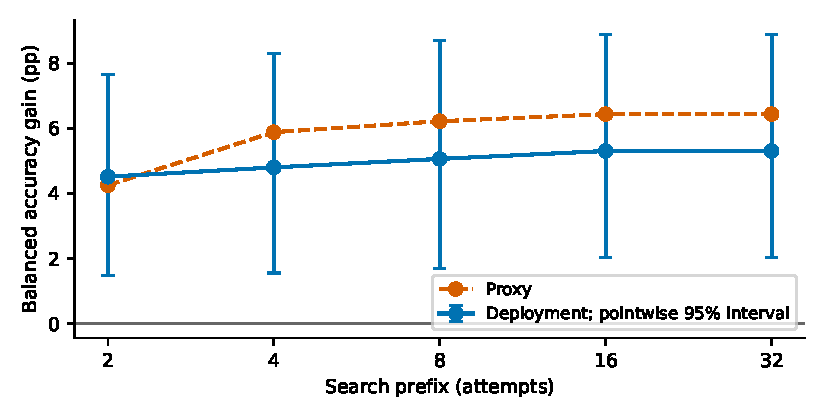
\includegraphics[width=.86\linewidth]{planner_prefix.pdf}
\caption{The bounded planner-code case. Gains are balanced-accuracy percentage points. Deployment intervals are exploratory crossed root/task bootstrap intervals over three generation roots and the fixed 20-task panel. The intervals are pointwise and do not test the difference between prefixes.}
\end{figure}
Nested prefixes reuse the same generation sequence, including invalid attempts. Selection uses four proxy tasks and a no-update option. A fixed menu and at most two training/finish actions bound the candidate programs. These constraints make the case interpretable but sharply limit claims about tool-using or autonomous research agents. No shared numerical stress scale is assumed between this study and market execution.

\section{Review and provenance limits}
The original freeze, implementation audit, saved-outcome reanalysis, and current manuscript audit are distinct records. A new scope/version binds the present manuscript without rewriting historical experiment receipts. The absence of duplicate file hashes or long matching prose passages alone is not proof of semantic originality; the comparison also considers the claims, cohorts, methods, and result sources.

Final authorship, conflicts, rights, and submission declarations require author confirmation. The paper's bounded scientific claims do not certify completion of the broader project or guarantee a venue decision. The review materials maintain anonymous authors and cite related work substantively.
\bibliographystyle{style/tmlr}
\bibliography{references}
\end{document}
